%
\documentclass{llncs}

\usepackage{graphicx}      % include this line if your document contains figures
%\usepackage{natbib}        % required for bibliography


\usepackage{amsmath} 

\usepackage{amssymb} 
%\newtheorem{thm}{Theorem}
 
\newtheorem{ex}{Exercise}

\newtheorem{expl}{Example}


\newtheorem{prop}{Proposition}

\newtheorem{thm}{Theorem}

\renewcommand{\today}{\number\month / \number\day / \number\year}
\pagestyle{plain}
\begin{document}

\title{Conformal flattening on the probability simplex and 
its applications to \\ 
%certain computational geometric problems}
Voronoi partitions and centroids}
%

\author{Atsumi Ohara}
%\inst{1} \and Roger Temam\inst{2} Jeffrey Dean \and David Grove \and Craig Chambers \and Kim~B.~Bruce \and Elsa Bertino} % \authorrunning{Ivar Ekeland et al.} % abbreviated author list (for running head) % %%%% list of authors for the TOC (use if author list has to be modified) 
%\tocauthor{Ivar Ekeland, Roger Temam, Jeffrey Dean, David Grove, Craig Chambers%, Kim B. Bruce, and Elisa Bertino} 
\institute{Department of Electrical and Electronics Engineering, 
University of Fukui \\ Bunkyo 3-9-1, Fukui 910-8507, Japan
\\ \email{ohara@fuee.u-fukui.ac.jp}
%,\\ WWW home page: bb
% \and Universit\'e de Paris-Sud, Laboratoire d'Analyse Num\'erique,\\
%F-91405 Orsay Cedex, France
}
%



\maketitle              % typeset the title of the contribution
%\footnote{printed on \today}
\begin{abstract}
A certain class of information geometric structure can be 
conformally transformed to dually flat one.
%Embedding or representing functions play important roles in order to produce
%various information geometric structure.
This paper studies the transformation on the probability simplex
from a viewpoint of {\em affine differential geometry} and provides 
its applications.
By restricting affine immersions with certain conditions,
the probability simplex is realized to be 1-conformally flat 
statistical manifolds immersed in ${\bf R}^{n+1}$.
Using this fact, we introduce a concept of {\em conformal flattening} 
for such manifolds in order to obtain the corresponding 
dually flat statistical (Hessian) ones with conformal divergences,
and show explicit forms of potential functions, dual coordinates.
Finally, we demonstrate applications of the flattening to
nonextensive statistical physics, Voronoi partitions and weighted centroids 
on the probability simplex with respect to {\em geometric divergences}, 
which is not necessarily of Bregman type.
\keywords{
Conformal flattening, Affine differential geometry, Escort probability, 
Geometric divergence, Conformal divergence
} 
\end{abstract}  


\section{Introduction}
In the theory of information geometry for statistical models,
the logarithmic function is crucially significant to give a standard 
information geometric structure for exponential family \cite{Amari85,AN}.
By changing the logarithmic
function to another one we can deform the standard structure 
to a new one while keeping its basic property as a statistical manifold, 
which consists of a pair of mutually dual affine connections 
$(\nabla, \nabla^*)$ with respect to Riemannian metric $g$.
There exist several ways \cite{Zhang04,Eguchi04,Naudts04,HSM14} 
to introduce functions to deform a statistical manifold 
structure and these functions are sometimes called 
{\em embedding} or {\em representing functions}. 

Affine immersion \cite{NS} can be regarded as one of possible ways.
Further, Kurose \cite{Kurose94} has proved that {\em 1-conformally flat} 
statistical manifolds (See Appendix) realized by 
a certain class of affine immersions can be conformally transformed to 
dually flat ones, which are the most fruitful 
information geometric structures. 

In this paper we call the transformation {\em conformal flattening} 
and give its explicit formula in order to 
elucidate the relations between representing functions and
realized information geometric structures.
We also discuss its applicability to 
computational geometric topics.
These are interpreted as generalizations of the results in \cite{OMA10,OMA12}, 
where the arguments are limited to conformal flattening of 
the alpha-geometry \cite{Amari85,AN} (See also section \ref{sec:example}).

The paper is organized as follows:
In section 2 we first discuss the affine immersion of 
the probability simplex and its geometric structure realized by
the associated {\em geometric divergence}. 
Next, the conformally flattening transformation is given and 
the obtained dually flat structure with 
the associated {\em conformal divergence} is investigated.
Section 3 describes applications of the conformal flattening.
We consider a Voronoi partition and a weighted centroid 
with respect to the geometric divergence on the probability simplex.
While geometric divergences are not of Bregman type in general, 
geometric properties such as conformality and projectivity are well utilized 
in these topics.
We also see that {\em escort probabilities}, 
which are interpreted as the dual affine coordinates for 
the flattened geometry, play important roles.
Section 4 includes concluding remarks.
Finally, a short review on statistical manifolds and 
affine differential geometry is given in Appendix.



%in order to elucidate a some aspects of geometrical meaning and properties.


%$(L, E), \ell, (L, E), (\Lambda, E), ({\cal L}, {\cal E})$
%
%{\bf Purpose:}
%\begin{itemize}
%\item When is a conformal change of geometrical divergence canonical?
%\item Explicit representation of potential functions and dual coordinates 
%in terms of a representing function $L$ (or immersion $f$) 
%and a transversal vector $\xi$.
%\end{itemize}

%\vspace{1em}
%\section{Preliminaries}
\section{Affine immersion of the probability simplex}
Let ${\cal S}^n$ be the relative interior of 
the probability simplex, i.e.,
\[
	{\cal S}^n :=\left\{p=(p_i) \left| 
		p_i \in {\bf R}_+, \; \sum_{i=1}^{n+1} p_i =1 \right.  \right\},
\]
where ${\bf R}_+$ denotes the set of positive numbers.

Consider an affine immersion \cite{NS}
$(f, \xi)$ of the simplex ${\cal S}^n$ (see also Appendix).
% that realizes $({\cal S}^n,\nabla,h)$.
%\;
%\noindent
%{\bf Definition}
Let $D$ be the canonical flat affine connection on ${\bf R}^{n+1}$.
Further, let 
$f$ be an immersion from ${\cal S}^n$ into ${\bf R}^{n+1}$ and 
$\xi$ be a transversal vector field on ${\cal S}^n$ (cf. figure 1).
For a given {\em affine immersion} $(f, \xi)$ of ${\cal S}^n$,
the induced torsion-free connection $\nabla$ 
and the affine fundamental form $h$ 
are defined from the Gauss formula by
\begin{equation}
	D_X f_*(Y)= f_*(\nabla_X Y)+h(X,Y)\xi,
		\quad X,Y \in {\cal X}({\cal S}^n),
\end{equation}
where $f_*$ is the differential of $f$ and 
${\cal X}({\cal S}^n)$ is the set of vector fields on ${\cal S}^n$.

It is well known \cite{Kurose94,NS} that the realized geometric structure 
$({\cal S}^n,\nabla,h)$ is a statistical manifold if and only if 
$(f, \xi)$ is nondegenerate and equiaffine, i.e., 
$h$ is nondegenerate and $D_X \xi$ is tangent to ${\cal S}^n$ for 
any $X \in {\cal X}({\cal S}^n)$.
Furthermore, the statistical manifold $({\cal S}^n,\nabla,h)$ is 
1-conformally flat \cite{Kurose94} 
(but not necessarily dually flat nor of constant curvature).

\begin{figure}[bhtp]
\vspace{0cm}
\begin{center}
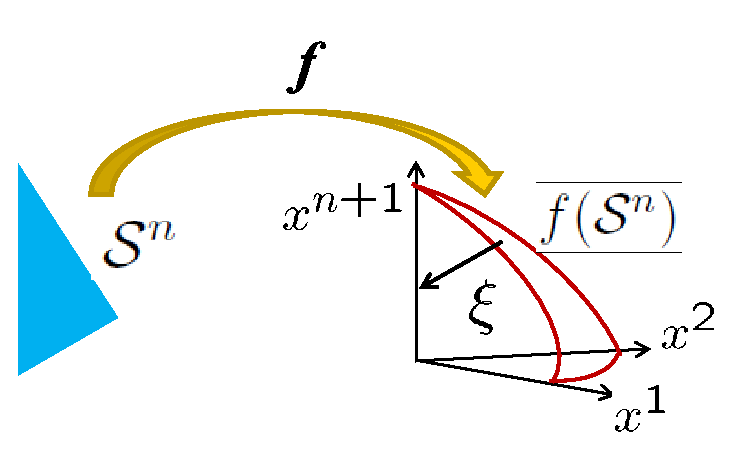
\includegraphics[width=10cm]{affine_im2.eps}
\caption{An affine immersion  $(f,\xi)$ from ${\cal S}^n$ to ${\bf R}^{n+1}$}
\end{center}
\end{figure}

Now we consider the affine immersion with the following assumptions.

\noindent 
{\bf Assumptions:}
\begin{enumerate}
\item The affine immersion $(f, \xi)$ is nondegenerate and equiaffine,
\item Let $\{x^i\}$ be an affine coordinate system for $D$ on 
${\bf R}^{n+1}$. 
The immersion $f$ is given by the component-by-component and 
a common representing function $L$, i.e., 
\[
%	f:{\cal S}^n \ni \bm{p}= (p_i) \mapsto \bm{x}=(x^i) \in {\bf R}^{n+1}, 
%	\quad x^i=L(p_i), \; i=1,\cdots,n+1, 
	f:{\cal S}^n \ni p= (p_i) \mapsto x=(x^i) \in {\bf R}^{n+1}, 
	\quad x^i=L(p_i), \; i=1,\cdots,n+1, 
\]
\item The representing function $L:(0,\;1) \rightarrow {\bf R}$ is 
sign-definite (or non-zero), 
concave with $L''<0$ and strictly increasing, i.e., $L' >0$,
Hence, the inverse of $L$ denoted by $E$ exists, i.e.,
$E \circ L ={\rm id}$.
\item Each component of $\xi$ satisfies $\xi^i <0, \; i=1,\cdots,n+1$ 
on ${\cal S}^n$.
% or $E=L^{-1}$.
\end{enumerate}
%Note that
%\begin{itemize}
%\item A statistical manifold $({\cal S}^n,\nabla,h)$ is 1-conformally flat  
%(, but not necessarily dually flat nor of constant curvature),
%\item $L$ is strongly concave or convex 
%$\Leftrightarrow$ there exists $\xi$, s.t. $h$ is positive definite,
%\item $E \circ L ={\rm id}$ implies that $ L' E' =1$.
%\end{itemize}

\begin{remark}
%We assume $L$ be strongly concave and strictly increasing, 
%i.e., $L''<0$ and $L' >0$.
%Then, 
From the assumption 3, it follows that 
$ L' E' =1$, $E'>0$ and $E''>0$.
Regarding sign-definiteness of $L$, note that 
we can adjust $L(u)$ to $L(u)+c$ by 
a suitable constant $c$ without loss of generality 
since the resultant geometric structure is unchanged 
(See Proposition \ref{prop:1}) by the adjustment.
For a fixed $L$ satisfying the assumption 3, 
we can choose $\xi$ that meets the assumptions 1 and 4.
For example, if we take $\xi^i=-|L(p_i)|$ then 
$(f,\xi)$ is called {\em centro-affine}, 
which is known to be equiaffine \cite{NS}.
%Note that $L$ is concave with $L'' <0$ or convex $L'' >0$ 
%if and only if there exists $\xi$ for $h$ to be positive definite.
The assumptions 3 and 4 also assure positive definiteness of $h$
(The details are described in the proof of Proposition \ref{prop:1}).
Hence, $(f,\xi)$ is non-degenerate and  
we can regard $h$ as a Riemannian metric on ${\cal S}^n$.
%{\bf This enables the assumption 4 holds.}
\end{remark}

\subsection{Conormal vector and the geometric divergence}
%\subsubsection{}
Define a function $\Psi$ on ${\bf R}^{n+1}$ by
\[
	\Psi(x):=\sum_{i=1}^{n+1} E(x^i),
\]
then $f({\cal S}^n)$ immersed in ${\bf R}^{n+1}$ 
is expressed as a level surface of $\Psi(x)=1$.
Denote by ${\bf R}_{n+1}$ the dual space of ${\bf R}^{n+1}$ and 
by $\langle \nu, x  \rangle$ the pairing of $x \in {\bf R}^{n+1}$ 
and $\nu \in {\bf R}_{n+1}$.
The conormal vector \cite{NS} $\nu: {\cal S}^n \rightarrow {\bf R}_{n+1}$ 
for the affine immersion $(f, \xi)$ is defined by
\begin{equation}
	\langle \nu(p), f_*(X) \rangle=0, \; \forall X \in T_p {\cal S}^n,
	\qquad \langle \nu(p), \xi(p)  \rangle =1
\label{conormal_vec}
\end{equation}
for $p \in {\cal S}^n$.
Using the assumptions and noting the relations:
\[
%\begin{equation}
	\frac{\partial \Psi}{\partial x^i}=E'(x^i)= \frac{1}{L'(p_i)}>0, \quad
	i=1,\cdots, n+1,
%\label{grad}
%\end{equation}
\]
we have 
%\[
\begin{equation}
	\nu_i(p):=\frac{1}{\Lambda} \frac{\partial \Psi}{\partial x^i}
	=\frac{1}{\Lambda(p)} E'(x^i)
	=\frac{1}{\Lambda(p)} \frac{1}{L'(p_i)}, \quad 	i=1,\cdots, n+1,
\label{comp_covec}
\end{equation}
%\]
where $\Lambda$ is a normalizing factor defined by
\begin{equation}
	\Lambda (p):=\sum_{i=1}^{n+1} \frac{\partial \Psi}{\partial x^i} \xi^i
	=\sum_{i=1}^{n+1} \frac{1}{L'(p_i)} \xi ^i(p).
\label{norm_factr}
\end{equation}
Then we can confirm (\ref{conormal_vec}) using 
the relation $\sum_{i=1}^{n+1} X^i =0$ for $X=(X^i) \in {\cal X}({\cal S}^n)$.
%\[
%	\langle \nu, \xi \rangle =1, \quad \langle \nu, f_* (X) \rangle =0,
%	\quad \forall X \in {\cal X}({\cal S}^n).
%\]
Note that $v: {\cal S}^n \rightarrow {\bf R}_{n+1}$ defined by
\[
	v_i(p):=\Lambda(p)\nu_i(p)=\frac{1}{L'(p_i)},  \quad i=1,\cdots,n+1,
\]
also satisfies 
\begin{eqnarray}
	\langle v(p), f_*(X) \rangle=0, \; \forall X \in T_p {\cal S}^n.
\label{orthogonal}
\end{eqnarray}
%Note that if we take each component of 
%the transversal vector $\xi^i, i=1,\cdots,n+1$ to be negative on ${\cal S}^n$,
%%\footnote{Is it a function of $p$?}
Further, 
it follows, from (\ref{comp_covec}), (\ref{norm_factr}) 
and the assumption 4, that
\[
	 \Lambda(p)<0, \quad \nu_i(p) <0,  \quad i=1,\cdots,n+1,
\]
for all $p \in {\cal S}^n$.

It is known \cite{NS} that the affine fundamental form $h$ can be 
represented by 
\[
	h(X,Y)=-\langle \nu_*(X),f_*(Y) \rangle, 
	\quad X,Y \in T_p{\cal S}^n.
\]
In our case, it is calculated via (\ref{orthogonal}) as
\begin{eqnarray*}
	h(X,Y)&=&-\Lambda^{-1} \langle v_*(X),f_*(Y) \rangle
		-X (\Lambda^{-1})\langle v,f_*(Y) \rangle \\
	&=&-\frac{1}{\Lambda} \sum_{i=1}^{n+1} 
		\left( \frac{1}{L'(p_i)} \right)' L'(p_i) X^iY^i 
	=\frac{1}{\Lambda} \sum_{i=1}^{n+1} \frac{L''(p_i)}{L'(p_i)}X^iY^i.
\end{eqnarray*}
Since $h$ is positive definite from the assumptions 3 and 4, 
we can regard it as a Riemannian metric.
%{\bf affine connection?}

Utilizing these notions from affine differential geometry,
we can introduce 
the function $\rho$ on ${\cal S}^n \times {\cal S}^n$, which is called 
a {\em geometric divergence} \cite{Kurose94}, as follows:
%A geometric divergence of $({\cal S}^n,\nabla,h)$ is 
\begin{eqnarray}
	\rho(p,r)&=&\langle \nu(r), f(p) - f(r) \rangle 
	= \sum_{i=1}^{n+1} \nu_i(r)(L(p_i) - L(r_i)) \nonumber \\
	&=& \frac{1}{\Lambda(r)} \sum_{i=1}^{n+1} 
		\frac{L(p_i) - L(r_i)}{L'(r_i)},
		\qquad p, r \in {\cal S}^n.
\label{geom_div}
\end{eqnarray}

We can easily see that $\rho$ is 
a contrast function \cite{Eguchi92,AN} of the geometric structure 
$({\cal S}^n,\nabla,h)$ because it holds that
\begin{eqnarray}
&	\rho[X|]=0, \quad h(X,Y)=-\rho[X|Y], &
\label{contrast_geometry1} \\
&	\quad h(\nabla_X Y,Z)=-\rho[XY|Z], \quad h(Y, \nabla^*_XZ)=-\rho[Y|XZ],
&
\label{contrast_geometry2}
\end{eqnarray}
where $\rho[X_1 \cdots X_k | Y_1 \cdots Y_l]$ stands for
\[
	\rho[X_1 \cdots X_k | Y_1 \cdots Y_l](p):=
		(X_1)_p \cdots (X_k)_p (Y_1)_r \cdots (Y_l)_r \rho(p,r)|_{p=r}
\]
for $p,r \in {\cal S}^n$ and $X_i, Y_j \in {\cal X}({\cal S}^n)$.

\subsection{Conformal divergence and 1-conformal transformation}
Let $\sigma$ be a positive function on ${\cal S}^n$.
Associated with the geometric divergence $\rho$, 
the {\em conformal divergence} \cite{Kurose94} of $\rho$ 
with respect to a conformal factor 
$\sigma(r)$ is defined by
\begin{equation}
	\tilde \rho(p,r)= \sigma(r) \rho(p,r), \qquad p, r \in {\cal S}^n.
\label{conf_div}
\end{equation}
The divergence $\tilde \rho$ can be proved  
to be a contrast function for $({\cal S}^n,\tilde \nabla, \tilde h)$, 
which is 1-conformally transformed geometric structure 
from $({\cal S}^n,\nabla,h)$,
where $\tilde h$ and $\tilde \nabla$ are given by
\begin{eqnarray}
	\tilde h&=& \sigma h, 
\label{CT_metric} 
\\
	h(\tilde \nabla_X Y, Z)&=& h(\nabla_X Y, Z)-d(\ln \sigma)(Z)h(X,Y).
\label{CT_conex}
\end{eqnarray}
When there exists such a positive function $\sigma$ that relates 
$({\cal S}^n,\nabla,h)$ with $({\cal S}^n,\tilde \nabla, \tilde h)$ as in 
(\ref{CT_metric}) and (\ref{CT_conex}), 
they are called 1-conformally equivalent and 
$({\cal S}^n,\tilde \nabla, \tilde h)$ is also a statistical manifold 
\cite{Kurose94}.

	
\subsection{Main result}

Generally, the induced structure $({\cal S}^n,\tilde \nabla, \tilde h)$ 
from the conformal divergence $\tilde \rho$ 
is not also dually flat, which is 
the most abundant structure in information geometry.
However, by choosing the conformal factor $\sigma$ carefully, 
we can demonstrate that $({\cal S}^n,\tilde \nabla, \tilde h)$ is dually flat. 
Hereafter, we call such a transformation as {\em conformal flattening}.

Define
\[
	Z(p):= \sum_{i=1}^{n+1} \nu_i(p)
	=\frac{1}{\Lambda(p)}\sum_{i=1}^{n+1} \frac{1}{L'(p_i)},
\]
then it is negative because each $\nu_i(p)$ is.
The conformal divergence of $\rho$ with respect to the conformal factor 
$\sigma(r):=-1/Z(r)$ is
\[
	\tilde \rho(p,r)= -\frac{1}{Z(r)}\rho(p,r).
\]
%which is positive, e.g., XXXX.
%
%Kurose \cite{} proved that $\tilde \rho$ is a contrast function 
%with respect to a statistical manifold 
%$({\cal S}^n,\tilde \nabla, \tilde h)$ defined by


\begin{proposition}
\label{prop:1}
If the conformal factor is given by $\sigma=-1/Z$, 
then the statistical manifold $({\cal S}^n,\tilde \nabla, \tilde h)$ 
that is 1-conformally transformed from $({\cal S}^n,\nabla,h)$ 
via (\ref{CT_metric}) and (\ref{CT_conex}) is dully flat.
Further, $\tilde \rho$ is the canonical divergence 
where mutually dual pair of affine coordinates $(\theta^i, \eta_i)$ 
and a pair of potential functions $(\psi, \varphi)$ are explicitly given by
\begin{eqnarray}
	\theta^i(p) &=& x^i(p)-x^{n+1}(p)=L(p_i)-L(p_{n+1}), \quad i=1,\cdots,n \\
	\eta_i(p) &=& \frac{\nu_i(p)}{Z(p)}=: P_i(p), \quad i=1,\cdots,n, \\
	\psi(p) &=& -x_{n+1}(p)=-L(p_{n+1}), \\
	\varphi(p) &=& \frac{1}{Z(p)} \sum_{i=1}^{n+1} \nu_i(p)x^i(p)
			= \sum_{i=1}^{n+1} P_i(p)L(p_i).
\end{eqnarray}
\end{proposition}
\begin{proof}
%Define functions $P_i$ on ${\cal S}^{n+1}$ by
%\[
%	P_i(p):=\frac{E'(x_i)}{\sum_{k=1}^{n+1} E'(x_k)}.
%\]
Using given relations, we first show that the conformal divergence 
$\tilde \rho$ is the canonical divergence \cite{AN} for 
$({\cal S}^n,\tilde \nabla, \tilde h)$:
\begin{eqnarray}
	\tilde \rho(p,r)&=& 
		-\frac{1}{Z(r)} \langle \nu(r), f(p) - f(r) \rangle
		= \langle P(r), f(r) - f(p) \rangle \nonumber \\
	&=& \sum_{i=1}^{n+1} P_i(r)(x^i(r) - x^i(p)) \nonumber \\
	&=& \sum_{i=1}^{n+1} P_i(r)x^i(r) 
		- \sum_{i=1}^{n} P_i(r)(x^i(p) - x^{n+1}(p))
		- \left(\sum_{i=1}^{n+1} P_i(r) \right)x^{n+1}(p) \nonumber \\
	&=& \varphi(r) - \sum_{i=1}^{n} \eta_i(r) \theta^i(p) + \psi(p).
\label{canonical}
\end{eqnarray}
Next, let us confirm that  
$\partial \psi/\partial \theta^i = \eta_i$.
Since $\theta^i(p)=L(p_i)+\psi(p), \; i=1,\cdots,n$, we have
\[
	p_i=E(\theta^i-\psi), \quad i=1,\cdots,n+1,
\]
by setting $\theta^{n+1}:=0$.
Hence, we have 
\[
	1= \sum_{i=1}^{n+1} E(\theta^i-\psi).
\]
Differentiating by $\theta^j$, we have
\begin{eqnarray*}
	0&=& \frac{\partial}{\partial \theta^j} 
			\sum_{i=1}^{n+1} E(\theta^i-\psi)
	=\sum_{i=1}^{n+1} E'(\theta^i-\psi) \left( \delta^i_j- 
		\frac{\partial \psi}{\partial \theta^j} \right) \\
	&=& E'(x^j) - \left( \sum_{i=1}^{n+1} E'(x^i) \right)
				\frac{\partial \psi}{\partial \theta^j}.
\end{eqnarray*}
This implies that
\[
	\frac{\partial \psi}{\partial \theta^j}
	=\frac{E'(x^j)}{\sum_{i=1}^{n+1} E'(x^i)}=P_j=\eta_j.
\]
Together with (\ref{canonical}) and this relation, 
$\varphi$ is confirmed to be the Legendre transform of $\psi$.

The dual relation $\partial \varphi/\partial \eta_i = \theta^i$ follows 
automatically from the property of the Legendre transform.
%$\psi=\varphi^*$ follows automatically? 
%(essentially smooth, Legendre type, Rockafeller)
\hfill Q.E.D.
\end{proof}

%\vspace{2mm}
\begin{remark}
\label{rem:rem2}
Since the conformal metric is $\tilde h=-h/Z$, 
it is also positive definite.
The dual affine connections $\nabla^*$ and $\tilde \nabla^*$ 
are known to be projectively equivalent \cite{Kurose94}. 
Hence, $\nabla^*$ is projectively (or $-1$-conformally) flat. 
% since $\tilde \nabla^*$ is flat.
%that the dual affine connections $\nabla^*$ and $\tilde \nabla^*$ 
%are projectively equivalent \cite{Kurose94}.
Further, the following corollary implies that 
the realized affine connection $\nabla$ is also projectively equivalent to
the flat connection $\tilde \nabla$ 
if we use the centro-affine immersion, 
i.e., $\xi^i=-L(p_i)$ \cite{NS,Kurose94} (See also Appendix).
Note that the expressions of the dual coordinates $\eta_i(p)=P_i(p)$ 
can be interpreted as a generalization of 
the {\em escort probability} \cite{Tsallis09} 
because it is a normalization of deformed probabilities $1/L'(p_i)$ 
(see the following subsection). 
\end{remark}
\begin{corollary}
The choice of $\xi$ does not affect the obtained dually flat structure 
$({\cal S}^n,\tilde \nabla, \tilde h)$.
\end{corollary}
\begin{proof}
We have the following alternative expressions of $\eta_i=P_i$ 
with respect to $L$ and $E$:
\[
	P_i(p)=\frac{1/L'(p_i)}{\displaystyle \sum_{k=1}^{n+1}1/L'(p_k)}
=\frac{E'(x_i)}{\displaystyle \sum_{i=1}^{n+1} E'(x_i)} >0, \quad i=1,\cdots,n.
\]
Hence, all the expressions in proposition 1 does not depend on $\xi$, and 
the statement follows.
\hfill Q.E.D.
\end{proof}

\subsection{Examples}
\label{sec:example}
{\bf Ex.1)} If we take $L$ to be the logarithmic function $L(t)=\ln (t)$, 
the conformally flattened geometry immediately defines 
the standard dually flat structure % \cite{AN}
$(g^{\rm F},\nabla^{(1)},\nabla^{(-1)})$ on the simplex ${\cal S}^n$,
where $g^F$ denotes the Fisher metric.
We see that $-\varphi(p)$ is the entropy, i.e., 
$\varphi(p)=\sum_{i=1}^{n+1} p_i \ln p_i$ and 
the conformal divergence is the KL divergence (relative entropy), i.e., 
$\tilde \rho(p,r)=D^{({\rm KL})}(r||p)=\sum_{i=1}^{n+1} r_i (\ln r_i-\ln p_i)$.

\noindent
{\bf Ex.2)} Next let the affine immersion $(f,\xi)$ be defined by 
the following $L$ and $\xi$:
\[
	L(t):=\frac{1}{1-q}t^{1-q}, \quad x^i(p)=\frac{1}{1-q}(p_i)^{1-q},
\]
and
\[
	\xi^i(p)=-q(1-q)x^i(p),
\]
with $0 <q$ and $q \not=1$, 
then it realizes the alpha-geometry \cite{AN}
$({\cal S}^n,\nabla^{(\alpha)}, g^F)$ with $q=(1+\alpha)/2$.
Since the immersion $(f, \xi)$ is centro-affine and the length of 
$\xi$ is suitably scaled, $({\cal S}^n,\nabla^{(\alpha)}, g^F)$ 
is of constant curvature $\kappa=(1-\alpha^2)/4$.
The associated geometric divergence is the alpha-divergence, i.e.,
\begin{equation}
	\rho(p,r)=D^{(\alpha)}(p,r)=\frac{4}{1-\alpha^2}
	\left(
	1-\sum_{i=1}^{n+1}(p_i)^{(1-\alpha)/2}(r_i)^{(1+\alpha)/2}
	\right).
\label{alpha_div}
\end{equation}
Following the procedure of conformally flattening  
described in the above, we have \cite{OMA10}
\[
	\Psi(x)=\sum_{i=1}^{n+1} ((1-q)x^i)^{1/{1-q}},
	\quad \Lambda(p)=-q, \; (constant) 
\]
\[
	\nu_i(p)=-\frac{1}{q}(p_i)^{q}, \quad 
	-\frac{1}{Z(p)}=\frac{q}{\sum_{k=1}^{n+1} (p_i)^q},
\]
and obtain dually flat structure 
$(\tilde h, \tilde \nabla, \tilde \nabla^*)$
via the formulas in proposition 1:
\[
	\eta_i=\frac{(p_i)^{q}}{\sum_{k=1}^{n+1}(p_k)^{q}}, \quad
	\theta^i=\frac{1}{1-q}(p_i)^{1-q} - \frac{1}{1-q}(p_{n+1})^{1-q}
	=\ln_q(p_i)-\psi(p),
\]
\[
	\psi(p)=-\ln_q(p_{n+1}), \quad 
	\varphi(p)=\ln_q \left( \frac{1}{\exp_q (S_q(p))} \right), \quad
	\tilde h(p)=-\frac{1}{Z(p)}g^F(p).
\]
Here, $\ln_q$ and $S_q(p)$ are the {\em q-logarithmic function} and 
the {\em Tsallis entropy} \cite{Tsallis09}, respectively defined by
\[
	\ln_q(t)=\frac{t^{1-q}-1}{1-q}, \quad 
		S_q(p)=\frac{\sum_{i=1}^{n+1}(p_i)^q -1}{1-q}.
\]

\section{Construction of Voronoi partitions 
and centroids with respect to geometric divergences}
In the previous section we have seen that various geometric divergences 
$\rho$ can be constructed on the statistical manifold ${\cal S}^n$ 
by changing the representing function $L$ and the transversal vector 
field $\xi$.

We demonstrate interesting applications of the conformal flattening to 
topics related with computational geometry, 
which are Voronoi partitions and centroids for the geometric divergence 
on a 1-conformally flat statistical manifold.
We find that escort probabilities $P_i$ (dual coordinates $\eta_i$) 
play important roles. 

In this section, subscripts by Greek letters such as $p_\lambda$  
are used to denote the $\lambda$-th point in ${\cal S}^n$ among given ones 
while subscripts by Roman letters such as $p_i$ denote 
the $i$-th coordinate of a point $p=(p_i) \in {\cal S}^n$.

\subsection{Voronoi partitions}

Let $\rho$ be a geometric divergence defined in (\ref{geom_div}) on a 
1-conformal statistical manifold $({\cal S}^n,\nabla, h)$.
For given $m$ points $p_\lambda, \; \lambda=1, \cdots, m$ on ${\cal S}^n$ 
we define {\em Voronoi regions} on ${\cal S}^n$ with respect to
the geometric divergence $\rho$ as follows:
\[
	{\rm Vor}^{(\rho)}(p_\lambda):=\bigcap_{\mu \not= \lambda} 
	\{ r \in {\cal S}^n | 
	\rho(p_\lambda,r)< \rho(p_\mu,r) \},
	\quad \lambda=1,\cdots,m.
\]
An {\em Voronoi partition (diagram)} on 
${\cal S}^n$ is a collection of the Voronoi regions and their boundaries.
For example, if we take $L(t)=t^{1-q}/(1-q)$ as in section \ref{sec:example}, 
the corresponding Voronoi partition is the one with respect to the 
alpha-divergence $D^{(\alpha)}$ in (\ref{alpha_div}) on 
$({\cal S}^n, \nabla^{(\alpha)},g^F)$ (Cf. the figures in \cite{OMA12} ).
Note that $D^{(\alpha)}$ approaches the Kullback-Leibler (KL) divergence 
if $\alpha \rightarrow -1$, and $D^{(0)}$ is called 
the Hellinger distance.
Further, the partition is also equivalent to that with respect to 
{\em R\'enyi divergence} \cite{Renyi} % of order}% $\alpha \not=1$ 
defined by
\[
	D_\alpha(p,r):= \frac{1}{\alpha-1} \ln 
		\sum_{i=1}^{n+1} (p_i)^{\alpha} (r_i)^{1-\alpha}
\]
because of their one-to-one functional relationship.

The acclaimed algorithm using projection of 
a convex polyhedron \cite{ES,Ed} has been known to commonly work well 
to construct Voronoi partitions for the KL divergence \cite{OT,OI,II} 
as well as the Euclidean distance.
Furthermore, the algorithm is generally applicable 
if a divergence function $\delta$ is of {\it Bregman type} \cite{NBN}, 
which is represented by 
the remainder of the first order Taylor expansion of 
a convex potential function in a suitable coordinate system.
Geometrically speaking, this implies that 
\begin{description}
\item[i)] the divergence $\delta$ is a {\em canonical divergence} \cite{AN} 
associated with a dually flat structure, i.e, it is of Bregman type: 
\begin{eqnarray}
	\delta (p,r)
	&=& \psi(\theta(r))+\varphi(\eta(r))
	-\sum_{i=1}^n \theta^i(p) \eta_i(r) \nonumber \\
	&=& \varphi(\eta(r))-\left\{ \varphi(\eta(p)) +\sum_{i=1}^n 
	\theta^i (p)\left( \eta_i(r)-\eta_i(p) \right) \right\}, 
\label{Bregman} \\
	&& \theta^i=\frac{\partial \varphi(\eta)}{\partial \eta_i}, \quad
	i=1,\cdots,n,
	\nonumber
\end{eqnarray}
\item[ii)] its affine coordinate system $\eta=(\eta_i)$ is chosen 
to realize the corresponding Voronoi partitions.
In this coordinate system with one extra complementary coordinate 
the polyhedron is expressed as the upper envelope of 
%an arrangement composed by 
$m$ hyperplanes tangent to the potential function $\varphi(\eta)$ 
at $\eta(p_\lambda), \; \lambda=1,\cdots,m$.
%See the cases of the Euclidean distance \cite{Ed}, 
%the Kullback-Leibler \cite{OI} and Bregman divergences \cite{NBN},
%respectively.
\end{description}

Unfortunately a problem for the case of our Voronoi partition is that 
the geometric divergences $\rho$ on ${\cal S}^n$ is {\em not} 
of Bregman type generally, i.e., they {\em cannot} be represented 
as a remainder of any convex potentials as in (\ref{Bregman}).

The following theorem, however, claims that the problem is resolved via  
Proposition 1. 
In other words, we can still apply the projection algorithm 
by conformally flattening a statistical manifold 
$({\cal S}, \nabla, h)$ 
to a dually flat structure $({\cal S}, \tilde \nabla,\tilde h)$ and 
by invoking the conformal divergence $\tilde \rho$, which is always 
of Bregman type, 
and escort probabilities $\eta_i(p)=P_i(p)$ as a coordinate system. 

The similar result is proved in \cite{OMA12} for the case of 
the $\alpha$-divergence $D^{(\alpha)}$.
However, the proof there was based on the fact that 
$({\cal S}^n,\nabla^{(\alpha)},g^F)$ is a statistical manifold {\em of 
constant curvature} in order to use 
the {\em modified Pythagorean relation} (See Appendix).
In the following theorem,  
the assumption is relaxed to a 1-conformally flat 
statistical manifold $({\cal S}, \nabla, h)$ and 
we prove with the usual Pythagorean relation on dually flat space.

Here, we denote the space of escort distributions by ${\cal E}^n$ and 
represent the point on ${\cal E}^n$ by $P=(P_1,\cdots,P_n)$ because 
$P_{n+1}=1-\sum_{i=1}^n P_i$ and ${\cal E}^n$ is also the probability 
simplex.

\begin{theorem}
\begin{description}
%\begin{romanlist}
\item{i)} The bisector of two points $p_\lambda$ and $p_\mu$ defined by 
$\{r |\rho(p_\lambda,r)=\rho(p_\mu,r)\}$ 
is a simultaneously $\nabla^*$- and $\tilde \nabla^*$-autoparallel 
hypersurface on ${\cal S}^n$.
%which is represented as  hyperplane on ${\cal E}^n$.
\item{ii)} 
Let ${\cal H}_\lambda, \lambda=1,\cdots,m$ be the hyperplane in 
${\cal E}^n \times {\bf R}$ which is respectively tangent 
at $(P(p_\lambda),  \varphi(p_\lambda))$ to the hypersurface 
$\{(P,y)=(P(p), \varphi(p)) | p \in {\cal S}^n \}$. %, where $p_\lambda=p(p_\lambda)$.
The Voronoi partition with respect to $\rho$
can be constructed on ${\cal E}^n$ by projecting 
the upper envelope of all ${\cal H}_\lambda$'s 
along the $y$-axis.
%the arrangement in ${\cal E}^n \times {\bf R}$ composed by .
%\end{romanlist}
\end{description}
\end{theorem}
%\noindent
%Proof) 
\begin{proof}
i) We construct a bisector for points $p_\lambda$ and $p_\mu$.
Consider the $\tilde \nabla$-geodesic $\tilde \gamma$ 
connecting $p_\lambda$ and $p_\mu$, and 
let $\bar{p}$ be the midpoint on $\tilde \gamma$ satisfying 
$\tilde \rho(p_\lambda,\bar{p})=\tilde \rho(p_\mu,\bar{p})$.
Note that the point $\bar{p}$ satisfies 
$\rho(p_\lambda,\bar{p})=\rho(p_\mu,\bar{p})$ 
by the conformal relation (\ref{conf_div}). 
Denote by ${\cal B}$ the $\tilde \nabla^*$-autoparallel hypersurface 
that is orthogonal to $\tilde \gamma$ at $\bar{p}$ 
with respect to the conformal metric $\tilde h$.
Note that ${\cal B}$ is simultaneously $\nabla^*$-autoparallel because of the 
projective equivalence of $\nabla^*$ and $\tilde \nabla^*$ as is 
mentioned in Remark \ref{rem:rem2}.

Using these setup and the fact that 
$({\cal S}^n, \tilde \nabla, \tilde h)$ is dually flat, 
we have the following relation from the Pythagorean theorem \cite{AN}
\[
	\tilde \rho(p_\lambda,r)=\tilde \rho(p_\lambda,\bar{p})+\tilde \rho(\bar{p},r)
	=\tilde \rho(p_\mu,\bar{p})+\tilde \rho(\bar{p},r)
	=\tilde \rho(p_\mu,r),
\]
for all $r \in {\cal B}$.
Using the conformal relation (\ref{conf_div}) again, 
we have $\rho(p_\lambda,r)=\rho(p_\mu,r)$ for all $r \in {\cal B}$.
Hence, ${\cal B}$ is a bisector of $p_\lambda$ and $p_\mu$.

ii) Recall 
%the equality $D^{(\alpha)}(p,r)=D^{(-\alpha)}(r,p)$ and 
the conformal relation (\ref{conf_div}) 
between $\rho$ and $\tilde \rho$, then we see that 
${\rm Vor}^{(\rho)}(p_\lambda)={\rm Vor}^{(\tilde \rho)}(p_\lambda)$ 
holds on ${\cal S}^n$, where 
\[
	{\rm Vor}^{(\tilde \rho)}(p_\lambda):=\bigcap_{\mu \not= \lambda} 
	\{ r \in {\cal S}^n | 
	\tilde \rho(p_\lambda,r)< \tilde \rho(p_\mu,r) \}.
\]
Proposition 1 and the Legendre relations (\ref{canonical}) 
%and (\ref{first_der})  
imply that $\tilde \rho(p_\lambda,r)$ 
is represented with the escort probabilities, i.e., 
the dual coordinates $(P_i)=(\eta_i)$ by
\[
	\tilde \rho(p_\lambda,r)=\varphi(P(r))
	-\left( \varphi(P(p_\lambda)) 
	+ \sum_{i=1}^n \frac{\partial \varphi}{\partial P_i} (p_\lambda)
	\{P_i(r) - P_i(p_\lambda)\} \right),
\]
%where $p=p(p)$.
%Note that a point $(P(r),y_\lambda(r))$ in ${\cal H}_\lambda$ is expressed by
%represent the hyperplane that is tangent at $(p_i,  \psi^*(p_i))$,
%where
By definition the hyperplane ${\cal H}_\lambda$ is expressed by
\[
	{\cal H}_\lambda=\left\{(P(r),y(r)) \left|\; y(r)= \varphi(P(p_\lambda)) 
	+ \sum_{i=1}^n \frac{\partial \psi^*}{\partial P_i} (p_\lambda)
	\{P_i(r) - P_i(p_\lambda)\}, \; r \in {\cal S}^n \right. \right\}.
\]
%\[
%	y_\lambda(p):= \varphi(p_\lambda) 
%	+ \sum_{i=1}^n \frac{\partial \psi^*}{\partial P_i} (p_\lambda)
%	\{P_i(r) - P_i(p_\lambda) \}.
%\]
Hence, we have $\tilde \rho(p_\lambda,r)=\varphi(P(r))-y(r)$.
Thus, we see, for example, that the bisector on ${\cal E}^n$ for 
$p_\lambda$ and $p_\mu$ is represented as a projection of 
${\cal H}_\lambda \cap {\cal H}_\mu$.
Thus, the statement follows.
\hfill Q.E.D.
\end{proof}

%\medskip
As a special case of the above theorem for $\rho=D^{(\alpha)}$, 
examples of Voronoi partitions with respect to $D^{(\alpha)}$ on 
usual probability simplex ${\cal S}^n$ and escort probability simplex 
${\cal E}^n$ are given with their figures in \cite{OMA12}.

%\begin{figure}[bhtp]
%\vspace{0cm}
%\begin{center}
%\centerline{\psfig{file=figure2.eps,width=15cm}}
%%\includegraphics[width=15cm]{figure2.eps}
%\caption{An example of $\alpha$-Voronoi diagram on ${\cal S}^2$ (left) 
%for $\alpha=-0.6$ (or $q=0.2$) and the corresponding one on ${\cal E}^2$ 
%(right).} 
%\centerline{\psfig{file=figure3.eps,width=15cm}}
%%\includegraphics[width=15cm]{figure3.eps}
%\caption{An example of $\alpha$-Voronoi diagram on ${\cal S}^2$ (left) 
%for $\alpha=2$ (or $q=1.5$) and the corresponding one on ${\cal E}^2$ 
%(right).} 
%\end{center}
%\end{figure}


\medskip
%\noindent
\begin{remark} 
Voronoi partitions for broader class of divergences 
that are not necessarily associated with any convex potentials are 
theoretically studied \cite{Matsu2} from more general 
affine differential geometric points of views.
%The construction algorithm is also given there,  
%if the suitable coordinates to realize it are explicitly identified.

On the other hand, if the domain is extended from ${\cal S}^n$ 
to the positive orthant ${\bf R}_+^{n+1}$, 
then the $\alpha$-divergence there can be expressed 
as a Bregman divergence \cite{Amari85,AN,Ohara07}.
Hence, the $\alpha$-geometry on ${\bf R}_+^{n+1}$ is dually flat.
Using this property, $\alpha$-Voronoi partitions on ${\bf R}_+^{n+1}$ is 
discussed in \cite{NN}.

However, while both of the above mentioned methods require 
constructions of the convex polyhedrons in the space of dimension $d=n+2$, 
the new one proposed in this paper does in the space of dimension $d=n+1$.
Since it is known \cite{Chaz} that 
the optimal computational time of polyhedrons 
depends on the dimension $d$ by $O(m\log m+m^{\lfloor d/2 \rfloor})$, 
the new one is slightly better when $n$ is even and $m$ is large.
%slightly better.
\end{remark}

\medskip

\subsection{Weighted Centroids}

Let $p_\lambda, \; \lambda=1, \cdots, m$ be given $m$ points 
on ${\cal S}^n$ and $w_\lambda > 0, \; \lambda=1, \cdots, m$ be their weights.
Define the {\em weighted $\rho$-centroid} $c^{(\rho)} \in {\cal S}^n$ by 
the minimizer of the following problem:
\[
	\min_{p \in {\cal S}^n} 
		\sum_{\lambda=1}^m w_\lambda \rho(p,p_\lambda).
\]
\begin{theorem}
The weighted $\rho$-centroid $c^{(\rho)}$ for given $m$ points 
$p_1, \cdots, p_m$ on ${\cal S}^n$ is expressed by 
\[
	P_i(c^{(\rho)})= \frac{1}{\sum_{\lambda=1}^m w_\lambda Z(p_\lambda)} 
		\sum_{\lambda=1}^m w_\lambda Z(p_\lambda) P_i(p_\lambda), 
		\quad i=1,\cdots,n+1,
\]
with weights $w_\lambda$, escort probabilities $P(p_\lambda)$ and 
the conformal factors $\sigma(p_\lambda)=-1/Z(p_\lambda)>0$ 
for $p_\lambda, \; \lambda=1,\cdots,m$.
\end{theorem}
%\noindent
%Proof) 
\begin{proof}
Denote $\theta^i(p)$ by $\theta^i$ simply. Using (\ref{conf_div}), 
%and the relation $D^{(\alpha)}(p,r)=D^{(-\alpha)}(r,p)$
we have
\begin{eqnarray*}
	\sum_{\lambda=1}^m w_\lambda \rho(p,p_\lambda)
	&=&-\sum_{\lambda=1}^m w_\lambda Z(p_\lambda)
		\tilde \rho(p,p_\lambda) \\
	&=&-\sum_{\lambda=1}^m w_\lambda Z(p_\lambda)\left\{\psi(\theta)
	+\psi^*(\eta(p_\lambda))
	-\sum_{i=1}^n \theta^i \eta_i(p_\lambda)\right\}.
\end{eqnarray*}
Then the optimality condition is 
\[
	\frac{\partial}{\partial \theta^i} 
	\sum_{\lambda=1}^m w_\lambda \rho(p,p_\lambda)
	= -\sum_{\lambda=1}^m w_\lambda Z(p_\lambda)
	\{\eta_i-\eta_i(p_\lambda)\}=0, 
	\quad i=1,\cdots, n,
\]
where $\eta_i=\eta_i(p)$.
Thus, the statements for $i=1,\cdots,n$ hold from $\eta_i=P_i$ in 
Proposition \ref{prop:1}.
For $i=n+1$, we have as follows:
\begin{eqnarray*}
	P_{n+1}(c^{(\rho)})&=&1-\sum_{i=1}^n P_i(c^{(\rho)}) \\
	&=&\frac{1}{\sum_{\lambda=1}^m w_\lambda Z(p_\lambda)} 
		\sum_{\lambda=1}^m w_\lambda Z(p_\lambda) 
		\left\{1-\sum_{i=1}^n P_i(p_\lambda) \right\}\\
	&=&\frac{1}{\sum_{\lambda=1}^m w_\lambda Z(p_\lambda)} 
		\sum_{\lambda=1}^m w_\lambda Z(p_\lambda) P_{n+1}(p_\lambda).
\end{eqnarray*}
\hfill Q.E.D.
\end{proof}

\section{Concluding remarks}
We have realized 1-conformally flat structures $({\cal S}^n,\nabla,h)$ by 
changing affine immersions $(f,\xi)$ or representing functions $L$, 
considered their conformal flattening and explicitly derived 
the corresponding dually flat structure, 
i.e., mutually dual potentials and affine coordinate systems.

Applications of the conformal flattening to topics in computational geometry 
are also demonstrated.
As a result the geometric divergence, 
which is not generally of Bregman type, 
can be easily treated via the traditional computation algorithm. 
Recently, conformal divergences for Bregman-type divergences are 
proposed from different viewpoints 
and their properties are exploited \cite{NN15,NNA16}.

Extensions of the conformal flattening to other non-flat statistical manifolds 
or families of continuous probability distributions 
are left in the future work.
While relations with the gradient flows (replicator flows, in a special case) 
on $({\cal S}^n,\nabla,h)$ or $({\cal S}^n,\tilde \nabla, \tilde h)$ 
can be found in \cite{Ohara18}, searching for the other applications 
of the technique would be also of interest.




%
% ---- Bibliography ----
%
\section*{Acknowledgements}
A. O. is partially supported by JSPS Grant-in-Aid (C) 15K04997.

\begin{thebibliography}{5}
%
\bibitem{Amari85} 
	Amari, S.-I.
	{\it Differential-Geometrical Methods in Statistics}, 
	Lecture Notes in Statistics, vol. 28, Springer, New York, (1985).
\bibitem{AN}
S-I. Amari and H. Nagaoka,
Methods of Information Geometry,
Trans. Math. Monogr. vol 191
(American Mathematical Society and Oxford University Press) (2000).
\bibitem{Shima07}
	Shima, H.
	{\em The geometry of Hessian structures},
	World Scientific, Singapore (2007).
\bibitem{NS}
K. Nomizu and T. Sasaki,
Affine Differential Geometry, Cambridge University Press,
Cambridge, (1993).

\bibitem{Kurose94}
T. Kurose, 
On the divergences of 1-conformally flat statistical manifolds,
Tohoku Math. J. 46, 427--433 (1994).

\bibitem{Zhang04}
J. Zhang
Divergence Function, Duality, and Convex Analysis,
Neural Computation 16, 159--195 (2004).

\bibitem{Eguchi04}
S. Eguchi,
Information geometry and statistical pattern recognition,
Sugaku Expositions,19, 197--216 (2006),
(originally 2004 Sugaku 56 380--99 in Japanese).

\bibitem{Naudts04}
J. Naudts, 
Continuity of a class of entropies and relative entropies,
Reviews in Mathematical Physics, 16, 6, 809--822 (2004).

\bibitem{HSM14}
K. V. Harsha and K. S. Subrahamanian Moosath, 
F-geometry and Amari's $\alpha$-geometry on a statistical manifold,
Entropy, 16(5), 2472--2487 (2014).
\bibitem{Eguchi92}
S. Eguchi,
Geometry of minimum contrast,
Hiroshima Math. J. 631-647 (1992).

\bibitem{OMA10}
A. Ohara, H. Matsuzoe and S.-I. Amari, 
A dually flat structure on the space of escort distributions
J. Phys.: Conf. Ser. 201, 012012 (2010).

\bibitem{OMA12}
A. Ohara, H. Matsuzoe and S. Amari,
Conformal geometry of escort probability and its applications,
Modern Physics Letters B, 26, 10 1250063 (14 pages) (2012).

\bibitem{Tsallis09}
C. Tsallis, 
Introduction to Nonextensive Statistical Mechanics: 
Approaching a Complex World, Springer, New York (2009).

%\bibitem{HS} J. Hofbauer and K. Sigmund,
%		The theory of evolution and dynamical systems : 
%		mathematical aspects of selection, 
%		{\it Evolutionary Games and Population Dynamics}, 
%		Cambridge University Press (1988).
\bibitem{Renyi} A. R\'enyi,
		On measures of entropy and information 
		{\it Proc. 4th Berkeley Symp. Math. Statist. Probability}
		{\bf 1} (Univ. Calif. Press: Berkeley, 547-561 (1961).
\bibitem{ES}	H. Edelsbrunner and R. Seidel,
		Voronoi diagrams and arrangements,
		{\it Discrete Comput. Geom.} {\bf 1}, 25-44 (1986).
\bibitem{Ed}	H. Edelsbrunner,
		{\it Algorithms in Combinatorial Geometry}
		Springer-Verlag, (1987).
\bibitem{OT}	K. Onishi and N. Takayama,
		Construction of Voronoi diagram on the Upper Half-Plane
		{\it IEICE Trans. on Fundamentals}, {\bf E79-A}, 
		533-539 (1996).
\bibitem{OI}	K. Onishi and H. Imai,
		Voronoi diagram in statistical parametric space by 
		Kullback-Leibler divergence,
		{\it Proc. 13th ACM-SIAM Symposium on Computational Geometry}, 
		 463-465 (1997).
\bibitem{II}	H. Imai and M. Inaba,
		Divergence-Based Geometric Clustering and Its Underlying 
		Discrete Proximity Structures,
		{\it IEICE Trans. Inf. \& Syst.}, {\bf E83-D}, 27-35 (2000).
\bibitem{NBN}	J.-D. Boissonnat, F. Nielsen and N. Nock,
		Bregman Voronoi diagram,
		{\it Discrete Comput. Geom.}, {\bf 44}, 281-307 (2010). 
\bibitem{Matsu2} H. Matsuzoe,
		Computational Geometry from the Viewpoint of Affine 
		Differential Geometry,
		{\it F.Nielsen eds. Emerging Trends in Visual Computing}, 
		Berlin/Heidelberg: Springer, 103-123 (2009).
\bibitem{Ohara07} A. Ohara,
		Geometry of distributions associated with Tsallis statistics
		and properties of relative entropy minimization,
		{\it Physics Letters}, A 370 (2007) 184-193.
\bibitem{NN}	F. Nielsen and R. Nock,
		The dual Voronoi diagrams with respect to representational 
		Bregman divergences,
		International Symposium on Voronoi Diagrams (ISVD), 
		DTU Lyngby, Denmark (IEEE Press, New York, 2009).
\bibitem{Chaz} B. Chazelle, 
		An optimal convex hull algorithm in any fixed dimension,
		{\it Discrete and Computational Geometry} {\bf 10}, 377-409 
		(1993).
\bibitem{NN15} F. Nielsen and R. Nock,
		Total Jensen divergences: definition, properties 
		and clustering, 
		IEEE International Conference on Acoustics, Speech and 
		Signal Processing (ICASSP) (2015).
\bibitem{NNA16} R. Nock, F. Nielsen, S.-I. Amari,
		On Conformal Divergences and their Population Minimizers
		{\em IEEE Trans. IT}, 62, 1, 527-538 (2016).
\bibitem{Ohara18} A. Ohara,
		Conformal flattening for deformed information geometries on 
		the probability simplex,
		Entropy, 20, 186 (2018).
\end{thebibliography}

\appendix

\section{A short review of statistical manifolds and affine differential geometry}
We shortly summarize the basic notions and results in information geometry 
\cite{Amari85,AN}, Hessian domain \cite{Shima07} 
and affine differential geometry \cite{NS,Kurose94}, 
which are used in this paper.
See for the details and proofs in the literature.

\subsection{Statistical manifolds}
For a torsion-free affine connection $\nabla$ and a pseudo-Riemannian 
metric $g$ on a manifold $\mathcal{M}$, the triple $(\mathcal{M},\nabla,g)$ 
is called a {\em statistical (Codazzi) manifold} if 
%$\nabla g$ is symmetric.
it admits another torsion-free affine connection $\nabla^*$ satisfying
\begin{equation}
 Xg(Y,Z)=g(\nabla_X Y, Z)+g(Y, \nabla^*_X Z)
\label{dualistic}
\end{equation}
for arbitrary $X,Y$ and $Z$ in ${\mathcal X}(\mathcal{M})$, where ${\mathcal X}(\mathcal{M})$ is the set of all tangent vector fields on $\mathcal{M}$.
We say that $\nabla$ and $\nabla^*$ {\em duals} of each other 
with respect to $g$, and $(g,\nabla,\nabla^*)$ is called 
{\em dualistic structure} on $\mathcal{M}$.

A statistical manifold $(\mathcal{M},\nabla,g)$ is said to be of 
{\em constant curvature} $\kappa \in {\bf R}$ 
if the curvature tensor $R$ of $\nabla$ satisfies
\begin{equation}
 R(X,Y)Z=\kappa \{g(Y,Z)X-g(X,Z)Y\}.
\label{smcc}
\end{equation}
When the constant $\kappa$ is zero, the statistical manifold is called
{\em flat}, or {\em dually flat}, because the dual curvature tensor $R^*$ 
of $\nabla^*$ also vanishes automatically \cite{AN,Shima07}.

For $\alpha \in \mathbf{R}$, statistical manifolds 
$(\mathcal{M},\nabla,g)$ and $(\mathcal{M},\tilde \nabla ,\tilde g)$ 
are said to be
{\em $\alpha$-conformally equivalent} \cite{Kurose94}
if there exists a positive function $\sigma$ on $\mathcal{M}$ satisfying
\begin{eqnarray*}
  \tilde g(X,Y)&=&\sigma g(X,Y) 
\label{conf_eq1} \\
 g( \tilde \nabla_X Y,Z)&=&g(\nabla_X Y,Z)
	-\frac{1+\alpha}{2}(d \ln \sigma)(Z)g(X,Y) \nonumber \\
 && +\frac{1-\alpha}{2}\{(d\ln \sigma)(X)g(Y,Z)+(d\ln \sigma)(Y)g(X,Z)\}.
\label{conf_eq2}
\end{eqnarray*}
Statistical manifolds $(\mathcal{M},\nabla,g)$ and 
$(\mathcal{M},\tilde \nabla, \tilde g)$ are $\alpha$-conformally
equivalent if and only if $(\mathcal{M},\nabla^*,g)$ and 
$(\mathcal{M},{\tilde \nabla}^*,\tilde g)$ are 
$-\alpha$-conformally equivalent.
In particular, $-1$-conformal equivalence means 
{\em projective equivalence} of $\nabla$ and $\tilde \nabla$, 
which implies that a $\nabla$-pregeodesic curve is 
simultaneously $\tilde \nabla$-pregeodesic \cite{NS}.
A statistical manifold $(\mathcal{M},\nabla,g)$ is called
{\em $\alpha$-conformally flat} if it is locally
$\alpha$-conformally equivalent to a flat statistical manifold.
It is known that a statistical manifold is of constant curvature 
if and only if it is $\pm 1$-conformally flat,
when dim $\mathcal{M} \ge 3$ \cite{Kurose94}.
%Statistical manifold of dimension greater than three 
%has constant curvature if and only if it is $\pm 1$-conformally
%flat \cite{Kurose94}.

\subsection{Affine differential geometry}
Let $\mathcal{M}$ be an $n$-dimensional manifold and consider 
an {\em affine immersion} \cite{NS} $(f,\xi)$, which is the pair of 
an immersion $f$ from $\mathcal{M}$ into $\mathbf{R}^{n+1}$ and a
transversal vector field $\xi$ along $f({\cal M})$. 
By a given affine immersion $(f,\xi)$ of $\mathcal{M}$ and the usual
flat affine connection $D$ of $\mathbf{R}^{n+1}$, the Gauss and Weingarten
formulas are respectively obtained as follows:
\begin{eqnarray*}
 D_Xf_*(Y) &=& f_*(\nabla_X Y) + h(X,Y)\xi, \\
 D_X \xi &=&- f_*(SX) + \tau(X) \xi.
\end{eqnarray*}
Here, $\nabla, h, S$ and $\tau$ are called, respectively, 
{\em induced connection, affine fundamental form, affine shape operator} 
and {\em transversal connection form}.
In this case, we say that the affine immersion realizes
$(\mathcal{M},\nabla,h)$ in $\mathbf{R}^{n+1}$.
If $h$ is non-degenerate (resp. $\tau=0$ on ${\cal M}$), 
the affine immersion $(f, \xi)$ is called 
{\em non-degenerate} (resp. {\em equiaffine}).
It is known that non-degenerate and equiaffine $(f,\xi)$ realizes  
a statistical manifold $({\cal M},\nabla,h)$ by regarding 
$h$ as a pseudo-Riemannian metric $g$.


 
%induced connection $\nabla$ and the affine fundamental form $h$ are determined
%by
%\[
% (x^*D)_X(x_*Y)=x_*(\nabla_X Y) + h(X,Y)\xi,
%\]
%where $D$ is the standard affine connection of $\mathbf{R}^{n+1}$ and
%$X,Y$ in $\mathcal{X}(\mathcal{M})$.

%Kurose \cite{Kurose94} proved 
Such a statistical manifold is characterized as follows:
\begin{proposition} \cite{Kurose94}
\label{Tohoku}
A simply connected statistical manifold
$(\mathcal{M},\nabla,g)$ can be realized by a non-degenerate and 
equiaffine immersion 
%with $\tilde{\nabla}=\nabla$, $h=g$ and $\tau =0$ 
if and only if it is 1-conformally flat. 
%When dim $\mathcal{M} \ge 3$, the statistical manifold is of 
%constant curvature if and 
%only if it is $\pm 1$-conformally flat.
%Further, the realized statistical manifold has constant curvature $c$ 
%if and only if $S=kI$.
\end{proposition}

Let a point $o$ in ${\bf R}^{n+1}$ be chosen as origin and 
consider an immersion $f$ from ${\cal M}$ to 
${\bf R}^{n+1} \backslash \{ o \}$ so that $\xi=-\overrightarrow{of(p)}$ is 
transversal to $f({\cal M})$ for $p \in {\cal M}$.
Such an affine immersion $(f,\xi)$ 
is called {\em centro-affine}, where 
the Weingarten formula is $D_X \xi =- f_*(X)$, 
or $S= I$ and $\tau=0$.
This implies that a centro-affine immersion, if it is non-degenerate, 
realizes a statistical manifold of constant curvature  
because of the Gauss equation:
\[
	R(X,Y)Z=h(X,Z)SX-h(X,Z)SY.
\]
Further, the realized affine connection $\nabla$ is projectively flat \cite{NS}.

Denote the dual space of ${\bf R}^{n+1}$ by ${\bf R}_{n+1}$ and 
the pairing of $x \in {\bf R}^{n+1}$ and $y \in {\bf R}_{n+1}$ by 
$\langle y, x \rangle$.
Define a map $\nu: {\cal M} \rightarrow {\bf R}_{n+1} \backslash \{o\}$ 
as follows:
\[
	\langle \nu_p, \xi_p \rangle =1, \quad 
	\langle \nu_p, f_*(X) \rangle =0 \quad (\forall X \in T_p {\cal M}).
\]
Such $\nu_p$ is uniquely defined and is called the {\em conormal vector}.

The pair $(\nu, -\nu)$ can be regarded as a centro-affine immersion 
from ${\cal M}$ into 
the dual space ${\bf R}_{n+1}$ equipped with the usual flat connection $D^*$.
The formulas are
\begin{eqnarray*}
	D^*_X(\nu_* Y)&=&\nu(\nabla^*_X Y)+h^*(X,Y)(-\nu), \\
	D^*_X (-\nu) &=& - \nu_*(X), 
\end{eqnarray*}
where $h^*(X,Y)=h(SX,Y)$, and $\nabla^*$ is dual of 
$\nabla$ with respect to $h$.
Hence, when $(f,\xi)$ realizes a statistical manifold $({\cal M}.\nabla,h)$ 
with $S=I$, then 
$(\nu, -\nu)$ realizes its dual statistical manifold 
$({\cal M}, \nabla^*, h)$ \cite{NS}.
Both manifolds are of constant curvature.

%, i.e., (\ref{dualistic}) holds where 
%$g$ is replaced by $h$.

For a statistical manifold $({\cal M}, \nabla,h)$ realized by 
a non-degenerate and equiaffine immersion $(f,\xi)$, 
we can define a {\em contrast function} $\rho$
that induces the structure $({\cal M}, \nabla,h)$
\[
	\rho(p,q)=\langle \nu(q), f(p)-f(q) \rangle, \quad (p,q \in {\cal M}).
\]
The function $\rho$ is called the {\em geometric divergence} of 
$({\cal M}, \nabla,h)$ \cite{Kurose94}.
For a statistical manifold $({\cal M},\tilde \nabla, \tilde h)$ that is 
1-conformally equivalent to $({\cal M}, \nabla,h)$, one of 
its contrast function is given by $\tilde \rho(p,q)=\sigma(q) \rho(p,q)$ 
for a certain positive function $\sigma$.
The contrast function $\tilde \rho$ is called the 
{\em conformal divergence} \cite{Kurose94}.

A statistical manifold $(\mathcal{M}, \nabla, g)$ of constant
curvature $\kappa$ is studied from a viewpoint of affine differential geometry 
\cite{Kurose94}.
It is known that $(\mathcal{M},\nabla,g)$ realized in $\mathbf{R}^{n+1}$ 
has the following geometric properties:
\begin{description}
 \item[P1] For three points $p,q$ and $r$ in ${\cal M}$ let 
the $\nabla$-geodesic connecting $p$ and $q$ and 
the $\nabla^*$-geodesic connecting $q$ and $r$ are 
orthogonal at $q$. 
Then the following modified Pythagorean relation holds:
\[
	\rho(p,r)=\rho(p,q)+\rho(q,r)-\kappa \rho(p,q)\rho(q,r),
\]
 \item[P2] An arbitrary $\nabla$-geodesic on $\mathcal{M}$ is the intersection of a two-dimensional subspace in $\mathbf{R}^{n+1}$ and $\mathcal{M}$,   
 \item[P3] The volume element $\theta$ on ${\cal M}$ induced 
from $\mathbf{R}^{n+1}$ satisfies $\nabla \theta =0$, 
\end{description}
and so on. 
A typical example of the statistical manifold of non-zero constant curvature 
is the alpha-geometry $({\cal S}^n,\nabla^{(\alpha)},g^F)$, where 
$\kappa=(1-\alpha^2)/4$.
In this case, the modified Pythagorean relation induces 
the widely-known nonextensivity relation of
Tsallis entropy \cite[Remark 2]{Ohara07}. 


%See for details  \cite{Kurose94,NS}.

\end{document}